\documentclass{article}
\usepackage[utf8]{inputenc}
\usepackage{hyperref}
\usepackage{pdfrender,xcolor}
\usepackage{graphicx}

\usepackage{amsmath,amssymb,amsthm}
\usepackage{mathtools,graphicx,tikz-cd}
\usepackage{blindtext}
\usepackage[margin = 1.25 in]{geometry}
\usepackage{enumitem}
\usepackage{physics}

\usepackage{fancyhdr,accents,lastpage}
\pagestyle{fancy}
\setlength{\headheight}{25pt}

\newtheorem{theorem}{Theorem}[section]
\newtheorem{corollary}{Corollary}[theorem]
\newtheorem{lemma}[theorem]{Lemma}

\theoremstyle{definition}
\newtheorem{definition}{Definition}[section]

\theoremstyle{remark}
\newtheorem*{remark}{Remark}
\newtheorem{exercise}{Exercise}
\newtheorem{example}{Example}[definition]


\DeclareMathOperator{\ab}{ab}
\DeclareMathOperator{\area}{area}
\DeclareMathOperator{\Aut}{Aut}
\DeclareMathOperator{\BGL}{BGL}
\DeclareMathOperator{\Br}{Br}
\DeclareMathOperator{\card}{card}
\DeclareMathOperator{\ch}{ch}
\DeclareMathOperator{\Char}{char}
\DeclareMathOperator{\CHur}{CHur}
\DeclareMathOperator{\Cl}{Cl}
\DeclareMathOperator{\coker}{coker}
\DeclareMathOperator{\Conf}{Conf}
\DeclareMathOperator{\disc}{disc}
\DeclareMathOperator{\End}{End}
\DeclareMathOperator{\et}{\text{\'et}}
\DeclareMathOperator{\Fix}{Fix}
\DeclareMathOperator{\Gal}{Gal}
\DeclareMathOperator{\GL}{GL}
\DeclareMathOperator{\Hom}{Hom}
\DeclareMathOperator{\Hur}{Hur}
\DeclareMathOperator{\im}{im}
\DeclareMathOperator{\Ind}{Ind}
\DeclareMathOperator{\Inn}{Inn}
\DeclareMathOperator{\Irr}{Irr}
\DeclareMathOperator{\lcm}{lcm}
\DeclareMathOperator{\Mor}{Mor}
\DeclareMathOperator{\ord}{ord}
\DeclareMathOperator{\Out}{Out}
\DeclareMathOperator{\Perm}{Perm}
\DeclareMathOperator{\PGL}{PGL}
\DeclareMathOperator{\Pin}{Pin}
\DeclareMathOperator{\PSL}{PSL}
\DeclareMathOperator{\rad}{rad}
\DeclareMathOperator{\sgn}{sgn}
\DeclareMathOperator{\SL}{SL}
\DeclareMathOperator{\SO}{SO}
\DeclareMathOperator{\Sp}{Sp}
\DeclareMathOperator{\Spec}{Spec}
\DeclareMathOperator{\Spin}{Spin}
\DeclareMathOperator{\St}{St}
\DeclareMathOperator{\Surj}{Surj}
\DeclareMathOperator{\Syl}{Syl}
\DeclareMathOperator{\tame}{tame}

\newcommand{\eps}{\varepsilon}
\newcommand{\QED}{\hspace{\stretch{1}} $\blacksquare$}
\renewcommand{\AA}{\mathbb{A}}
\newcommand{\CC}{\mathbb{C}}
\newcommand{\EE}{\mathbb{E}}
\newcommand{\FF}{\mathbb{F}}
\newcommand{\HH}{\mathbb{H}}
\newcommand{\NN}{\mathbb{N}}
\newcommand{\OO}{\mathbb{O}}
\newcommand{\PP}{\mathbb{P}}
\newcommand{\QQ}{\mathbb{Q}}
\newcommand{\RR}{\mathbb{R}}
\newcommand{\ZZ}{\mathbb{Z}}
\newcommand{\bfm}{\mathbf{m}}
\newcommand{\mcA}{\mathcal{A}}
\newcommand{\mcC}{\mathcal{C}}
\newcommand{\mcG}{\mathcal{G}}
\newcommand{\mcH}{\mathcal{H}}
\newcommand{\mcM}{\mathcal{M}}
\newcommand{\mcN}{\mathcal{N}}
\newcommand{\mcO}{\mathcal{O}}
\newcommand{\mcP}{\mathcal{P}}
\newcommand{\mcQ}{\mathcal{Q}}
\newcommand{\mfa}{\mathfrak{a}}
\newcommand{\mfb}{\mathfrak{b}}
\newcommand{\mfI}{\mathfrak{I}}
\newcommand{\mfM}{\mathfrak{M}}
\newcommand{\mfm}{\mathfrak{m}}
\newcommand{\mfo}{\mathfrak{o}}
\newcommand{\mfO}{\mathfrak{O}}
\newcommand{\mfP}{\mathfrak{P}}
\newcommand{\mfp}{\mathfrak{p}}
\newcommand{\mfq}{\mathfrak{q}}
\newcommand{\mfz}{\mathfrak{z}}
\newcommand{\AGL}{\mathbb{A}\GL}
\newcommand{\Qbar}{\overline{\QQ}}
\renewcommand{\qedsymbol}{$\blacksquare$}
\renewcommand{\d}[1]{\ensuremath{\operatorname{d}\!{#1}}}

\pdfrender{StrokeColor=black,TextRenderingMode=2,LineWidth=0.5pt}

\lhead{\pdfrender{StrokeColor=black,TextRenderingMode=2,LineWidth=0.5pt}Number Theory} 
\chead{\pdfrender{StrokeColor=black,TextRenderingMode=2,LineWidth=0.5pt}Math Club}
\rhead{\pdfrender{StrokeColor=black,TextRenderingMode=2,LineWidth=0.5pt}Winter 2021} 


\begin{document}

\section{Introduction}

    Welcome to week 9 of math club!
    We've almost made it through the quarter, keep up the good work and good luck studying for your finals.
    Today we will be looking more at number theory, since it seems like A1 and B1 are commonly number theory questions.
    We will be looking at an important strategy to attack number theoretic problems rather than explicit theorems (for that, see last quarter's number theory sheet or use Google).
    I have also included some game theory problems that we didn't have time to get to last meeting in case anyone wants to try them out.

    Our main problem-solving strategy today is decomposition into primes.
    The general principle is this: to study the properties of a number, study the properties of each prime in its decomposition.
    Take this year's A1:
    \begin{exercise}[2020 A1]
        How many positive integers \(N\) satisfy all of the following three conditions?
        \begin{enumerate}
            \item[(i)] \(N\) is divisible by 2020.
            \item[(ii)] \(N\) has at most 2020 decimal digits.
            \item[(iii)] The decimal digits of \(N\) are a string of consecutive ones followed by a string of consecutive zeros.
        \end{enumerate}
    \end{exercise}
    As a helpful note, always know the prime factorizations of the current year and the ones adjacent: \(2020=2^2\cdot 5\cdot 101\), \(2021=43\cdot 47\), \(2022=2\cdot 3\cdot 337\).

    Resouces are the usual suspects and can be found on the Slack page.

\section{Problems}

    \begin{exercise}
        If \(17!=355687ab8096000\), find \(a\) and \(b\).
    \end{exercise}

    \begin{exercise}
        Prove that every 6-digit number of the form \(abcabc\) is divisible by 7, 11, and 13.
    \end{exercise}

\section{Leftover Game Theory}

\subsection{Chomp}

    In Chomp, you begin with a \(4\times 6\) (or in general \(n\times m\)) chocolate bar, and players alternate turns by chomping a square out of the chocolate bar, along with any squares that are to the right and above.
    However, the square in the lower left is poisoned!
    The player forced to chomp it loses.

    You can play against a bot here: \url{https://www.math.ucla.edu/~tom/Games/chomp.html}.
    You can play against another person controlled by you here: \url{https://www.geogebra.org/m/HSwgnXjn}.

    \begin{figure}[hbt!]
        \small
        \centering
        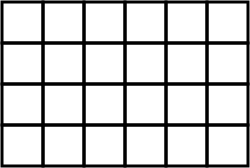
\includegraphics[scale = 0.4]{Pics/chomp.png}
    \end{figure}

    \begin{exercise}
        Determine which player wins as well as the winning strategy.
    \end{exercise}

\subsection{Sim}

    In Sim, six dots are drawn.
    Each dot is connected to every other dot by a line.
    Gameplay proceeds as follows.
    Players take turns coloring any uncolored lines.
    One player uses red, while another uses blue.
    Each player is trying to avoid creating a triangle made solely from their color; the player who completes such a triangle loses instantly.
    Also, only triangles whose vertices are among the six original dots count; intersections of lines don't matter.

    You can play the game here: \url{https://wideaperture.net/sim/}.

    \begin{figure}[hbt!]
        \small
        \centering
        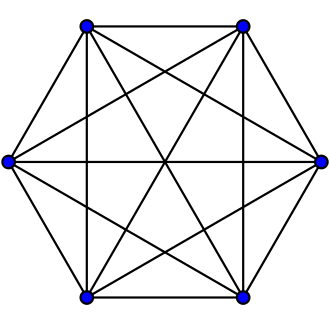
\includegraphics[scale = 0.4]{Pics/sim.png}
    \end{figure}

    \begin{exercise}
        Play the game and explore its properties.
        There are many connections between this game and Ramsey theory.
    \end{exercise}

\subsection{Miscellaneous}

    \begin{exercise}
        In a game of tic-tac-toe, suppose that the first player plays in the corner, and the second player does NOT play in the center.
        Prove that the first player can force a win.
    \end{exercise}

    \begin{exercise}[Bachet's Game]
        Initially there are \(n>0\) checkers on the table.
        The legal moves consist of removing at least one but not more than \(k<n\) checkers from the table.
        The winner is the one to take the last checker.
        For what values of \(n\) will the first person have the winning strategy?
        How about the second person?
        What are the losing positions?
    \end{exercise}

    \begin{exercise}
        Consider Bachet's Game again, but this time the legal moves consist of removing any power of 2 checkers.
        What is the winning strategy for the first and second player this time?
        What are the losing positions?
    \end{exercise}

    \begin{exercise}[2020 B2]
        Let \(k,n\in\ZZ\) with \(1\leq k<n\).
        Alice and Bob play a game with \(k\) pegs in a line of \(n\) holes.
        At the beginning of the game, the pegs occupy the \(k\) leftmost holes.
        A legal move consists of moving a single peg to any vacant hole that is further to the right.
        The players alternate moves, with Alice playing first.
        The game ends when the pegs are in the \(k\) rightmost holes, so whoever is next to play cannot move and therefore loses.
        For what values of \(n\) and \(k\) does Alice have a winning strategy?
    \end{exercise}

\end{document}